---
title: Higher Homotopy Groupoids
numbersections: true
---

\section{Preliminaries: Category Theory}

% TODO

\begin{thm}\label{functors-preserve-isomorphism}
	Let $F: C\rightarrow D$ be a functor, and $f: X\rightarrow Y$ a isomorphism in $C$. Then $F(f)$ is an isomorphism between $F(X)$ and $F(Y)$ in $D$.
\end{thm}

\begin{proof}
	Let $f^{-1}$ be the inverse of $f$. Then $$F(f^{-1})F(f) = F(f^{-1}f) = F(id_X) = id_{F(X)},$$ and the same works on the other side.
\end{proof}




\section{The Fundamental Groupoid}
\label{The Fundamental Group}

\begin{notation}
	When the context is unclear, we will call a general homotopy a \emph{free
		homotopy}, and a homotopy with fixed endpoints a \emph{path homotopy}.
\end{notation}

Before defining the fundamental groupoid, there is a nice geometric picture to
tell about the fundamental group. Fix a topological space $X$ and a point
$x_0$. Draw a representative of each of the non-identity homotopy classes of
loops at $x_0$, and note that each arrow is double-sided, since paths can be
traversed in either direction. When you "erase" the information of the
underlying space, you get a single point and a bunch of double-headed arrows:
exactly the "objects-and-arrows" picture of a group!

\begin{figure}[H]
	\centering
	\usetikzlibrary{decorations.markings}

\newcommand{\pathA}{(2, 2) .. controls (3,2) and (3, 1.5) .. (4, 1.5)}
\newcommand{\pathB}{(4, 1.5) .. controls (5, 1.5) and (5,2) .. (6, 2)}
\newcommand{\pathC}{(6, -2) .. controls (5,-2) and (5, -1.5) .. (4, -1.5)}
\newcommand{\pathD}{(4, -1.5) .. controls (3, -1.5) and (3,-2) .. (2, -2)}

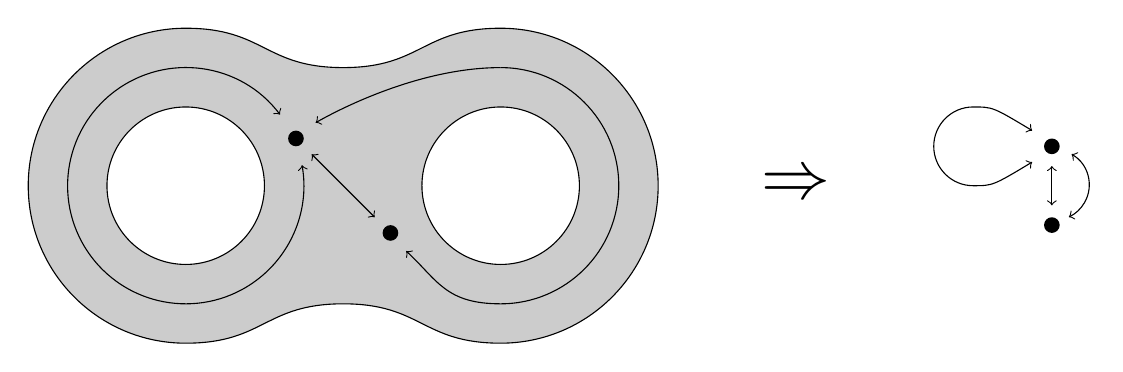
\begin{tikzpicture}
	% outer shape
	\filldraw[fill=black, fill opacity=0.2, draw=black] (0, 0) arc(180:90:2) --
	\pathA --
	\pathB --
	(6, 2) arc(90:0:2) --
	(8, 0) arc(360:270:2) --
	\pathC --
	\pathD --
	(2, -2) arc(270:180:2)
	;

	% inner holes
	\filldraw [fill=white] (2,0) circle (1);
	\filldraw [fill=white] (6,0) circle (1);

	% paths
	\coordinate (x) at (3.4, 0.6);
	\coordinate (y) at (4.6, -0.6);
	\node [circle, fill, inner sep=2pt] at (x) {};
	\draw[<->] ([shift=(37:1.5)]2,0) arc(37:370:1.5);
	\draw[<-] (3.65, 0.8) .. controls (4,1) and (5,1.5) .. (6, 1.5);
	\draw[<-] (4.8, -0.83) .. controls (5.2,-1.2) and (5.3, -1.5) .. (6, -1.5);
	\draw ([shift=(270:1.5)]6,0) arc(270:450:1.5);

	\node [circle, fill, inner sep=2pt] at (y) {};
	\draw[<->] (3.6, 0.4) -- (4.4, -0.4);

	\node[font={\Huge\Huge\bfseries\sffamily}] at (9.75, 0) {$\Rightarrow$};

	% the group!
	\coordinate (x) at (13, 0.5);
	\coordinate (y) at (13, -0.5);
	\node [circle, fill, inner sep=2pt] at (x) {};
	\node [circle, fill, inner sep=2pt] at (y) {};
	\draw[<->] (12.75, 0.7) .. controls (12.25,1.0) .. (12,1.0) --
	(12,1.0) arc(90:270:0.5) --
	(12,0) .. controls (12.25,0) .. (12.75, 0.3)
	;
	\draw[<->] (13.25, 0.4) arc (60:-65:0.45);
	\draw[<->] (13, 0.25) -- (13, -0.25);
\end{tikzpicture}

	\caption{Generators of the fundamental group on a two-holed disk.}
	\label{fig:group}
\end{figure}

% TODO: how does this motivate the groupoid

\begin{dfn}[Fundamental Groupoid]
	The \textit{fundamental groupoid} $\Pi_1(X)$ of a space $X$ is the category whose
	objects are points of $X$ and whose morphisms are path homotopy classes of
	paths in $X$.
\end{dfn}

Specifically, let $x,y,z\in X$, $f$ a path from $x$ to $y$, and $g$ a path from
$y$ to $z$. Then,

\begin{itemize}
	\item A path's domain is its source: $\text{dom}([f]) = x$.
	\item A path's codomain is its sink: $\text{cod}([f]) = y$.
	\item The identity is the constant map: $\id_x = [c_x]$.
	\item Composition is concatenation: $[g]\circ [f] = [f*g]$.
\end{itemize}

This construction is well-defined specifically because we are working with path
homotopies. For example, in general two paths with different sources may be
free homotopic, meaning without restricting to path homotopy we could not even
write down the domain and codomain of our morphisms.

\begin{ex}
	We can immediately compute a few examples of fundamental groupoids.
	\begin{itemize}
		\item The fundamental groupoid of a convex space is a \emph{tree groupoid},
		      i.e. a groupoid with precisely one morphism between any two objects.
		      This corresponds to the fact that any two paths with the same
		      endpoints in such a space are homotopic via the straight line
		      homotopy.
		\item The fundamental groupoid of a totally disconnected space is a
		      \emph{discrete groupoid}, i.e. a groupoid with only identity morphisms.
		      This corresponds to the fact that the only paths in such spaces are the
		      constant paths.
	\end{itemize}
\end{ex}

\begin{prop}\label{fund-is-groupoid}
	The fundamental groupoid is a groupoid.
\end{prop}

\begin{proof}
	All of this work was already done in class for the fundamental group. We restate the results here for groupoids.
	\begin{itemize}
		\item Composition is well-defined, since concatenation preserves homotopy equivalence.
		\item Composition is associative, since concatenation is associative up to homotopy.
		\item Every object $x$ has $[c_x]$ as an identity.
		\item Every morphism $[f]$ has $[\bar{f}]$ as an inverse.
	\end{itemize}

	The first three say that $\Pi_1(X)$ is a category, and the last says that it is a groupoid.
\end{proof}

The construction of the fundamental groupoid naturally gives rise to a functor
$$\Pi_1: \text{Top}\rightarrow\text{Grpd}.$$ In particular, let $f:
	X\rightarrow Y$ be a continuous function. We can view $f$ as acting on paths
via composition. Accordingly, we define
\begin{align*}
	\Pi_1(f)  \colon \Pi_1(X) & \to \Pi_1(Y)            \\
	[\gamma]                  & \mapsto [f\circ\gamma].
\end{align*}

This mapping is well-defined because composition preserves homotopy equivalence.

\begin{prop}\label{fund-is-functor}
	$\Pi_1$ is a functor.
\end{prop}

\begin{proof}
	Again, much of this work was done in class.
	\begin{itemize}
		\item $\Pi_1$ respects composition, since composition is associative.
		\item $\Pi_1$ respects the identity, since composing with the identity is
		      an identity up to homotopy. \qedhere
	\end{itemize}
\end{proof}

This result is an improvement over the fundamental group, where we needed a
functor out of based spaces for the definition to make sense. This is a first
hint that the fundamental groupoid in some sense captures more of the structure
of a space than the fundamental group does.

\begin{cor}\label{fund-is-topological}
	The fundamental groupoid is a topological invariant.
\end{cor}

\begin{proof}
	This follows from \Cref{functors-preserve-isomorphism} and \Cref{fund-is-functor}.
\end{proof}
